\chapter{État de l’art}
\section{Besoin d'explicabilité}
Expliquer les modèles de décisions boites noires est un besoin se faisant de plus en plus ressentir et suscitant de nombreux débats et tables rondes dans la communauté scientifique. Les entreprises recherchent avant toute chose la performance et ce au détriment de la transparence des algorithmes utilisés. En effet dans le domaine du machine learning il existe une multitude d'algorithmes pouvant être utilisés afin de fournir une prédiction, mais il existe une corrélation non négligeable entre les performances et la transparence de notre modèle comme le montre la figure 1.1. En général, plus notre modèle est performant, plus il est difficile à comprendre.\par

\begin{figure}[h]
\centering
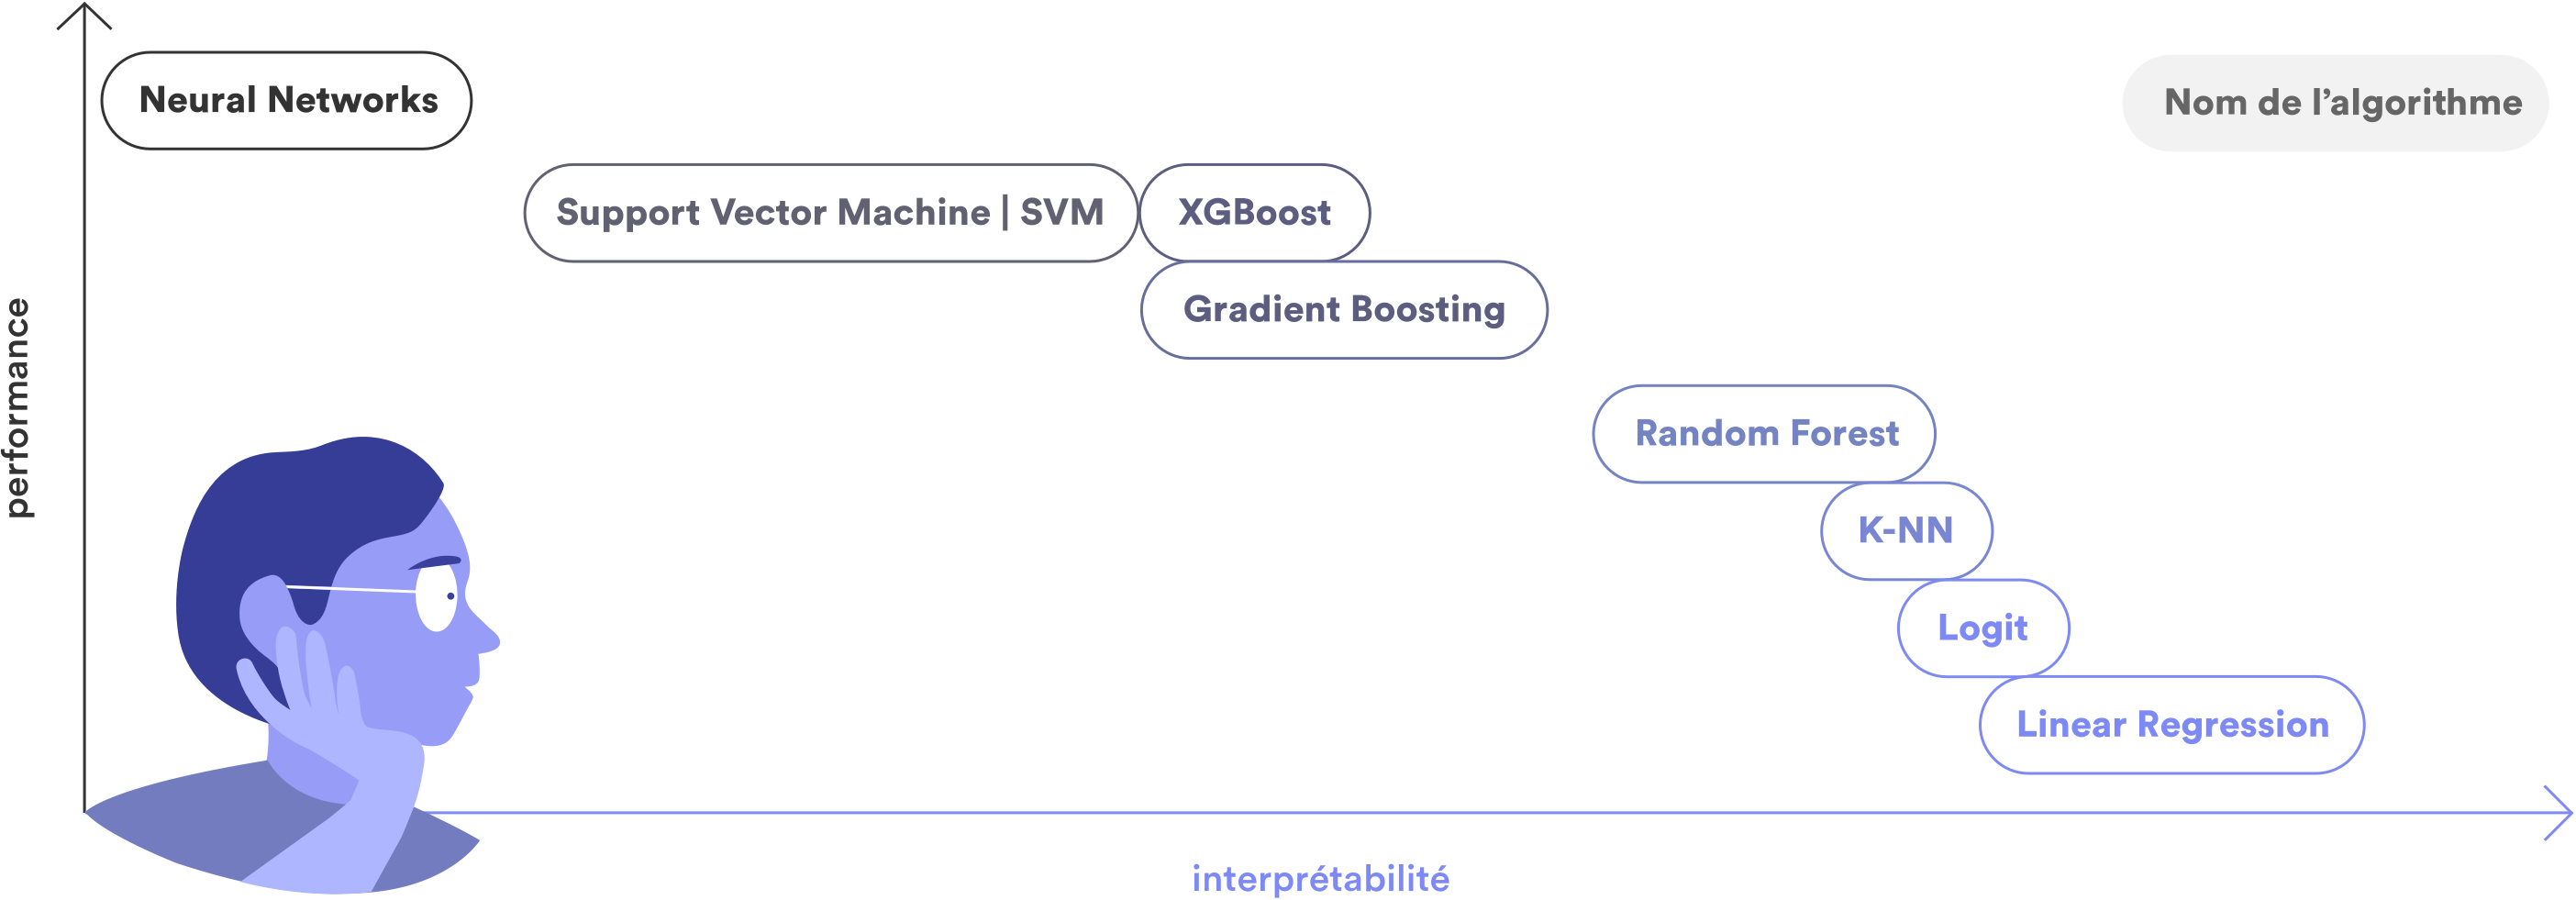
\includegraphics[scale=0.15]{src_img/performanceAndInterpretabilite.png}
\caption{Lien entre la performance et l'interprétabilité d'un algorithme de machine learning. \textit{Source : https://hippocrate.tech/}}
\label{performanceAndInterpretabilite}
\end{figure}

À l'heure actuelle, le réseau de neurones artificiel fait partie des algorithmes les plus performante et aussi est le plus couramment utilisée.
La non-explicabilité de ces modèles posent des problèmes de fiabilité, d'éthique et de responsabilité. Ce floue accentue aussi la méfiance et la peur des personnes envers l'intelligence artificielle, et entraîne un problème de compréhension entre les Data Scientist et les expert métier qui en plus de ne pas comprendre comment fonctionne le modèle ne comprennent pas non plus son résultat. Aussi, expliquer ces modèles permettrai d'améliorer notre conformité à la loi ainsi que d'augmenter les performances de nos modèles. Cette nouvelle problématique présente donc de nombreux enjeux de tailles.\par

\subsection{L'éthique}
Tout d'abord, de nombreux cas très exposés dans les médias nous montrent que cette incompréhension peut amener à des problèmes du point de vue éthique. La question de l'éthique est souvent ramenée à deux aspects principaux : la discrimination et la protection des données privées des usagers.
\subsubsection{La discrimination}
La question essentielle à se poser est de savoir comment une intelligence artificielle est amenée à prendre des décisions discriminante. Dans un article, Barocas et Selbst distinguent cinq façons par lesquelles une intelligence artificielle pourrait aboutir à une discrimination \cite{discriminationWay}. Ces cas sont uniquement des cas involontaires et ne prennent pas en compte une discrimination délibérée qui pourrait bien évidemment être possible.
\begin{itemize}
    \item \textbf{Définition des variables cibles et des étiquettes de classes} : le but d'une intelligence artificielle est de découvrir des corrélations dans des jeux de données. Ainsi, certain choix de variables cibles ou ou d'étiquettes de classes peuvent amener à faire des corrélations discriminatoire. Un exemple trivial serait de considérer un modèle permettant de savoir si un employé fait du travail de qualité, l'entreprise choisira de prendre en compte les retards des employés dans son modèle d'évaluation. Les personnes défavorisées habitant souvent loin de leur lieu de travail, ont plus souvent tendance à être en retard à cause des embouteillages et des problèmes de transport. Ces employés habitant loin, seront jugés comme faisant du travail de moins bonne qualité ce qui n'est pas forcément le cas. Si on ajoute à cela le fait que les personnes issus de l'immigration sont en moyenne plus pauvre et habitent en moyenne plus loin des centres villes, nous pouvons arriver involontairement à une IA discriminante par le simple fait d'utiliser l'étiquette "retard" dans l'évaluation des performances d'un employé.
    \item \textbf{Les données d'apprentissage} : les données d'apprentissage peuvent contenir des biais qui seront ensuite appris par notre modèle. L'exemple de l'IA de recrutement de l'entreprise Amazon qui rejetait les CVs contenant le mot "femme" évoqué en introduction le montre bien. Cette IA avait appris en analysant tous les profils recrutés par Amzon dans le passé, or les personnes recrutées étaient très majoritairement des hommes. L'IA a donc déduis qu'il était préférable de recruter des hommes. 
    \item \textbf{La collecte des données d'apprentissages} : Les lieux dans lesquels sont récoltées les données d'apprentissage sont aussi déterminant. Par exemple si l'on récolte des données concernant la criminalité dans un quartier avec des personnes issus majoritairement de l'immigration, l'IA aura plus tendance à considérer les immigrés comme de potentiels criminels par rapport aux personnes non-imigrées et inversement si on choisis un quartier avec des personnes majoritairement non-imigrées.
    \item \textbf{La sélection des caractéristiques} : Afin que l'IA puisse s'entraîner, il faut lui fournir des données qui sont en réalité une représentation simplifiée de notre monde. Ainsi, son créateur doit faire des choix pour sélectionner les caractéristiques qui constitueront cette représentation. Ce choix peut par concours de circonstance involontairement découler sur de la discrimination il faut donc les choisir avec parcimonie.
    \item \textbf{Données indirect} : Certaines données peuvent inclure des données indirect. Par exemple : \textit{"un jeu de données qui ne contient pas de données explicites sur l’orientation sexuelle peut tout de même la dévoiler. Une étude de 2009 a montré que les liens d’"amis" sur Facebook révèlent l’orientation sexuelle par une méthode de prédiction précise de l’orientation sexuelle des utilisateurs de Facebook fondée sur l’analyse de leurs liens. Le pourcentage d’"amis" s’identifiant comme homosexuels serait fortement corrélé avec l’orientation sexuelle de l’utilisateur concerné"}\footnote{Frederik Zuiderveen Borgesius, Discrimination, intelligence artificielle et décisions algorithmiques}. 
\end{itemize}
Mieux comprendre le fonctionnement de nos algorithmes permettrait donc de mieux se prémunir des discriminations involontaires. Aussi on pourrait prendre en compte l'explication en plus de la prédiction afin de fournir un résultat optimal. Par exemple, aux États-Unis, un algorithme appelé Compas est utilisé par les juges pour évaluer la probabilité pour un prévenu de se faire arrêter à nouveau dans les deux ans à venir. Cet algorithme est beaucoup remis en cause, car il est jugé "non-pertinant" et "discriminatoire" par certaines personnes alors que d'autres ont grandement confiance en lui, deux camps s'affrontent donc. Dans ce cas-là, fournir une explication conjointement à la prédiction permettrai de mettre tout le monde d'accord, ainsi nous pouvons prendre en compte la prévision et déterminer si dans le cas précis elle est issue d'un jugement non-pertinant, discriminatoire ou autre.
\subsubsection{Protection des données}
L'apprentissage d'une intelligence artificielle requière un très grand nombre de données, parmi lesquelles peuvent se trouver des données personnelles. L'utilisation d'un modèle pourrait donc aussi nécessiter de fournir des données personnelles afin d'effectuer une prédiction. L'utilisation de ces données jugées critiques est problématique, car des restrictions et des règles de protection en découlent. Tel qu'évoqué dans l'introduction, le RGPD par l'addition de plusieurs de ses articles implique un "droit à l'explication". Ce droit a été démontré par Seth Flaxman et Bryce Goodman \cite{RGPDexplanRight}, ce qui a donc pour effet d'accentuer le besoin d'applicabilité des modèles de décision boites noires. En effet, pour le moment ce droit est inaccessible par les usagers et les entreprises éprouvent des problèmes de responsabilités.

\subsection{Fiabilité et confiance}
Deuxièmement, expliquer les décisions prisent par un modèle boite noire permettrai d'augmenter la fiabilité que l'on lui accorde. Le modèle peut très bien fonctionner dans la plupart des cas, mais il est possible qu'il réagisse mal dans un certain cas bien spécifique. Avec l'absence de compréhension du fonctionnement interne de notre modèle, nous pouvons ne pas prévoir ce cas spécifique qui représente un risque. Le domaine médical par exemple est en attente d'une plus grande fiabilité de ses modèles en effet, une erreur peut avoir des conséquences graves et mettre en danger des personnes. La manière classique de mesurer la fiabilité d'un modèle est de calculer sa précision (accuracy), cela consiste à diviser le nombre de prédictions corrects par le nombre de prédiction total. Cette méthode indispensable ne permet pas à elle seule une fiabilité optimal en notre modèle, admettons que nous arrivons à une précision de 100\% rien ne nous dis que dans un cas très particulier notre modèle ne nous donnera pas une prédiction fausse. La compréhension de la logique interne de notre modèle serai donc un facteur supplémentaire dans la fiabilité que l'on lui donne. \par
De plus, un soudage publié par OpinionWay\footnote{https://www.opinion-way.com/fr/} montre que 30\% des Français ont peur d'un jugement porté par l'intelligence artificielle dans le domaine financier et 21\% dans le domaine médical. L'incompréhension de la logique interne des algorithmes décisionnels tend à accentuer la méfiance envers ces technologies. Fournir une explication permettrai d'augmenter l'acceptation de ces nouvelles technologies.

\subsection{Performance}
Enfin, expliquer la logique interne de la boite noire permettrai d'améliorer le développement de celle-ci, de la rendre plus compétitive et plus performante. Ces explications seront aussi utiles durant leur développement afin de comprendre pourquoi notre modèle ne fonctionne pas bien dans certains cas voir même pourquoi il ne converge pas du tout.

\section{Interprétabilité et explicabilité}

Dans le domaine du machine learning, les mots interprétabilité et explicabilité sont très souvent utilisés conjointement et il peut être difficile au premier abords d'en saisir la différence. De plus, il existe de nombreuses définitions différentes pour ces termes et tous les experts ne s'accordent pas forcement à ce sujet. Après l'analyse de différentes propositions, nous nous accorderons, dans ce mémoire, à donner les définitions suivantes :\par
L'interprétabilité est le fait de pouvoir observer l'effet d'une cause dans un système c'est-à-dire de pouvoir prédire les changements dans la sortie lorsque l'on change une variable d'entrée.\par
L'explicabilité, quant à elle, est le fait d'expliquer dans des termes compréhensibles par l'homme la mécanique interne de notre système.\par
Afin de bien saisir la différence, le site \textit{KDnuggets} dans un article du nom de "Machine Learning Explainability vs Interpretability: Two concepts that could help restore trust in AI"\footnote{https://www.kdnuggets.com/2018/12/machine-learning-explainability-interpretability-ai.html} nous invite à voir les choses comme si nous faisons une expérience scientifique à l'école : L'expérience peut être interprétable dans la mesure où vous pouvez voir ce que vous faites, mais elle n'est vraiment explicable qu'une fois que vous avez creusé la chimie derrière ce que vous pouvez voir se produire.\par
Créer un modèle interprétable implique de prendre en compte plusieurs facteurs :\par
\begin{description}
\item[Interprétabilité globale et local] L'interprétabilité d'un modèle est dite \textit{globale}, lorsque l'on comprend sa logique dans la totalité, nous sommes donc en mesure d'en expliquer toutes les solutions. À contrario, elle sera dite \textit{local}, lorsqu'il est possible d'expliquer seulement une ou plusieurs solutions spécifiques. Un problème complexe pourra ainsi être découpé en un sous problème plus simple afin de pouvoir expliquer une partie des solutions comme le montre la figure 1.2 ci-dessous.
\begin{figure}[h]
\centering
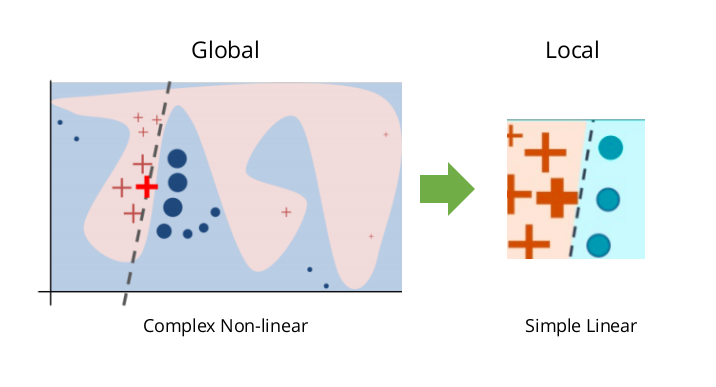
\includegraphics[scale=0.4]{src_img/globalVSlocal.png}
\caption{Un problème global complexe pouvant être expliqué à échelle local. \textit{Source : www.kdnuggets.com}}
\label{globalVSlocal}
\end{figure}

\item[Limatation temporel] Le temps que l'on peut allouer pour fournir une explication à notre modèle est aussi à prendre en compte. En effets, fournir une explication peut prendre du temps et cette explication peut être longue à appréhender pour un être humain. Dans certains contextes où la prise de décision devra être effectuée rapidement, il sera préférable d'avoir une explication simple, compréhensible et fournis rapidement par la machine. Dans d'autres cas, nous pourrons prendre le temps d'aborder une explication plus complexe et détaillée.

\item[La cible de l'explication] La nature de l'expertise de l'utilisateur est aussi un facteur à prendre en compte dans le choix de l'explication que nous voulons lui apporter. En effets, un expert dans le domaine aura tendance à préférer une explication exhaustive et précises qu'une explication simple et opaque et inversement pour une personne moins à l'aise.
\end{description}

\subsection{Pré-requis d'un modèle interprétable}
En plus de prendre en compte les facteurs précédemment évoqués, un modèle interprétable doit être capable de satisfaire une liste de choses souhaitées. L'article "A survey of methods for explaining black box models"\cite{surveyExplaining} met en avant, après une analyse de différents états de l'art traitant de ce sujet, les desiderata d'un modèle interpretable :
\begin{description}
\item[Interpretabilité] Dans quelle mesure le modèle ou la prédiction sont compréhensifs par l'homme. Ce sujet est encore en débat afin de savoir comment mesurer cette interprétabilité.

\item[Précision] Dans quelle mesure le modèle interprétable prédit avec précision les différentes instances. La précision d'un modèle peut être faite avec le \textit{score de précision} (accuracy score), il s'agit simplement d'un rapport entre les observations correctement prédites et les observations totales. La précision est l'indicateur de base afin de calculer la précision d'un modèle, ce score fonctionne mieux si les faux positifs et les faux négatifs ont un coût similaire. Si le coût des faux positifs et des faux négatifs est très différent, il vaut mieux regarder le \textit{F1-score}. Le F1-score est la moyenne pondérée de la précision et du rappel.
\[
F1 Score = 2*\frac{Recall * Precision}{Recall + Precision}
\]
Où la \textit{précision} est le rapport des observations positives correctement prédites au total des observations positives prévues. Et le \textit{recall} (rappel) est le rapport des observations positives correctement prédites à toutes les observations dans la classe réelle.

\item[Éthique] Si notre modèle traite des données personnelles, il devra garantir en plus une protection contre toutes formes de discrimination ainsi qu'une protection de la vie privée des personnes concernées.\\
\end{description}

Ces différents aspects jouent un rôle important quant à la confiance qu'un utilisateur va apporter à notre modèle interprétable. De plus d'autres notions viennent s'ajouter, notamment pour les modèles d'exploration de données et d'apprentissage automatique. Il est important de respecter des critères tels que la \textit{robustesse}, la \textit{causalité}, l'\textit{évolutivité} et la \textit{généralité}. Cela signifie qu'un modèle doit garantir un certain niveau de performance indépendamment des données d'entrée (robustesse), et que les changements d'entrée dû à une perturbation affectent le comportement du modèle (causalité). Enfin, étant donné que nous pouvons utiliser le même modèle avec une multitude données d'entrée et dans différents cas d'applications, il est préférable d'avoir des modèles portables possédant un minimum de restriction (évolutivité, généralité).

\section{Ouvrir les boites noires}
L'article "A survey of methods for explaining black box models"\cite{surveyExplaining} passe en revue cinquante-quatre méthodes aillant pour but d'ouvrir différentes boites noires, en nous fournissant une classification exposée dans un tableau disponible en annexe 1 et 2. Nous aurons l'occasion de reparler de ce tableau plus tard. Cette revue permet de distinguer différents types de problèmes, d'explicateurs, de boites noires, de données d'entrée ainsi que différentes restrictions sur le modèle (accès au code, aux données...). Nous allons commencer par expliquer ces différentes caractéristiques.

\subsection{Types de problèmes}
\subsubsection{Explication du modèle}
Ce problème consiste à fournir un modèle interprétable et transparent capable d'imiter le comportement d'une boite noire et de nous fournir un prédicat compréhensible par l'homme.\\
Étant donnée un prédicateur de boite noire b et un ensemble de données D, le problème d'explication du modèle consiste à trouver une fonction f telle que f(b,D)=c où c est un prédicateur compréhensible capable d'imiter le comportement de b et dérivable afin d'obtenir une explication.

\subsubsection{Explication du résultats}
Ce problème consiste à fournir un résultat interprétable, c'est-à-dire que le modèle devra fournir le résultat avec une explication sur les raisons qui l'ont poussé à donner cette prédiction. Il n'est pas nécessaire d'expliquer la logique interne du système mais seulement le processus de décision pour une instance donnée (interprétation local).

\subsubsection{Inspection de la boîte noire}
Ce problème consiste à fournir une représentation visuelle ou textuelle afin de comprendre le fonctionnement interne de notre boite noire.\\
Étant donnée un prédicateur de boite noire b et un ensemble de données D, le problème d'explication du modèle consiste à trouver une fonction f telle que f(b,D)=V où V est une représentation du fonctionnement de la boite noire.

\subsubsection{Conception transparente}
Ce problème consiste à fournir un modèle transparent qui soit directement interprétable globalement ou localement.

\subsection{Types d'explicateurs}
\begin{itemize}
    \item \textbf{Arbre de décision (Decision Tree)} : L'arbre de décision exploite un arbre qui a pour noeuds des conditions, les arrêtes correspondent à la valeur d'une variable d'entrée et les feuilles correspondent aux différents labels possible. La figure 1.3 montre un exemple trivial d'arbre de décision. Ainsi, la décision sera simplement expliquée en exprimant les chemins de l'arbre empruntés. 

    \begin{figure}[h]
    \centering
    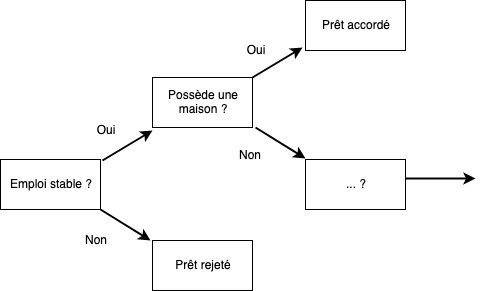
\includegraphics[scale=0.5]{src_img/decision_tree.jpg}
    \caption{Exemple d'un arbre de décision}
    \label{decision_tree}
    \end{figure}
    
    \item \textbf{Règles de décision (Decion Rules)} : Utilisé pour expliquer le modèle, le résultat ainsi que pour la conception transparente. Il est aussi possible de transformer un arbre en un ensemble de règles. Les règles de décisions sont simplement des conditions IF-THEN : 
    
    if condition1, condition2, condition3 then outcome 
    
    \item \textbf{Importance des fonctionnalités (Features Importance)} : Solution souvent utilisée, elle consiste à trouver les entrées de la boite noire pour lesquelles les poids sont les plus importants. Par exemple, pour une classification d'image, de trouver les pixels les plus importants dans l'entrée pour en arriver à une prédiction. Comme le montre la figure 1.4 tirée de l'article \textit{"Explainable Artificial Intelligence: Understanding, Visualizing and Interpreting Deep Learning Models"} \cite{explainingIA}.\\
    \begin{figure}[h]
        \centering
        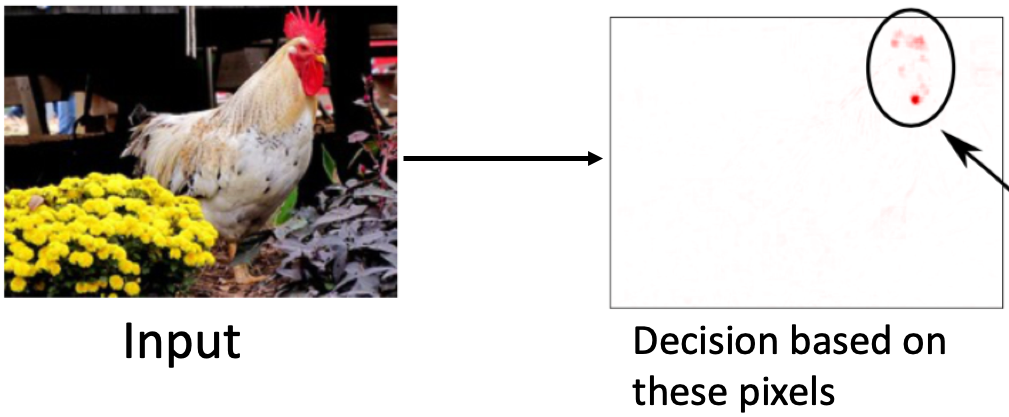
\includegraphics[scale=0.35]{src_img/chickenPixel.png}
        \caption{Importance des fonctionnalités : explication de la prédiction "coq"}
        \label{chickenPixel}
    \end{figure}
    
    \item \textbf{Salient Mask} Généralement utilisé pour expliquer localement les réseaux de neurones profond (DNN), le salient mask permet de mettre en évidence visuellement les parties déterminantes de l'entrée analysée. L'article \textit{"Real Time Image Saliency for Black Box Classifiers"}\cite{silentMask} décrit son fonctionnement et la figure 1.5 montrant un exemple de salient mask est tirée de cet article.
    \begin{figure}[h]
        \centering
        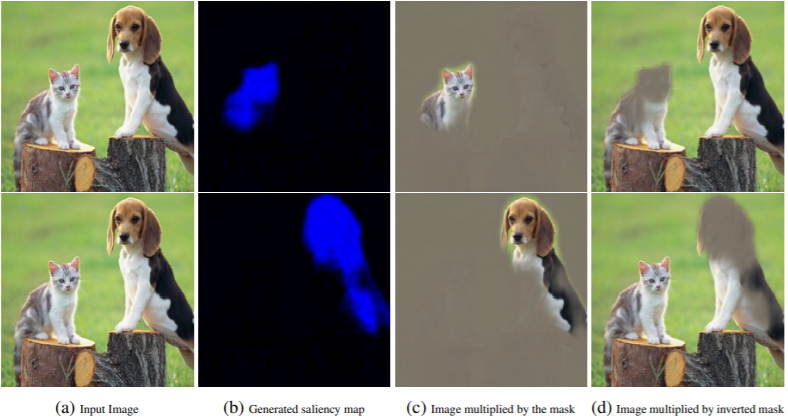
\includegraphics[scale=0.85]{src_img/silentMaskExemple.PNG}
        \caption{Masque saillant : explication de la prédiction chien et chat}
        \label{silentMaskExemple}
    \end{figure}
    
    \item \textbf{Analyse de sensibilité (Sensitivity Analysis)} : Généralement utilisée pour l'inspection de boite noire. L'analyse de sensibilité consiste à évaluer l’incertitude statistique du résultat d’une boîte noire avec les différentes sources d’incertitude dans ses entrés. En d'autres termes, cela consiste à modifier des variables d'entrées afin de voir si cela a un impact sur le résultat en sorti et donc de savoir comment elles affectent notre prédiction.
    
    \item \textbf{Diagramme de dépendance partielle (Partial Dependence Plot)} : Ces graphiques permettent de comprendre l'effet d'une ou deux variables d'entrée sur la sortie du modèle. Le but étant de  montrer si la relation entre une caractéristique d'entrée et la sortie est linéaire, monotone ou plus complexe. Par exemple, appliqué à un modèle de régression linéaire, les tracés de dépendance partielle montrent toujours une relation linéaire. Nous somme limité par une ou deux variables à la fois, car une variable donne une représentation en 2 dimensions du problème et deux variables fournissent donc une représentation 3 en dimensions. Par exemple, la figure 1.6 tirée du livre \cite{molnar2019} montre trois diagrammes de dépendances différents sur trois valeurs d'entrées (la température, l'humidité et la vitesse du vent) et leurs impactes linéaire sur la prédiction du nombre de vélos.
    \begin{figure}[h]
        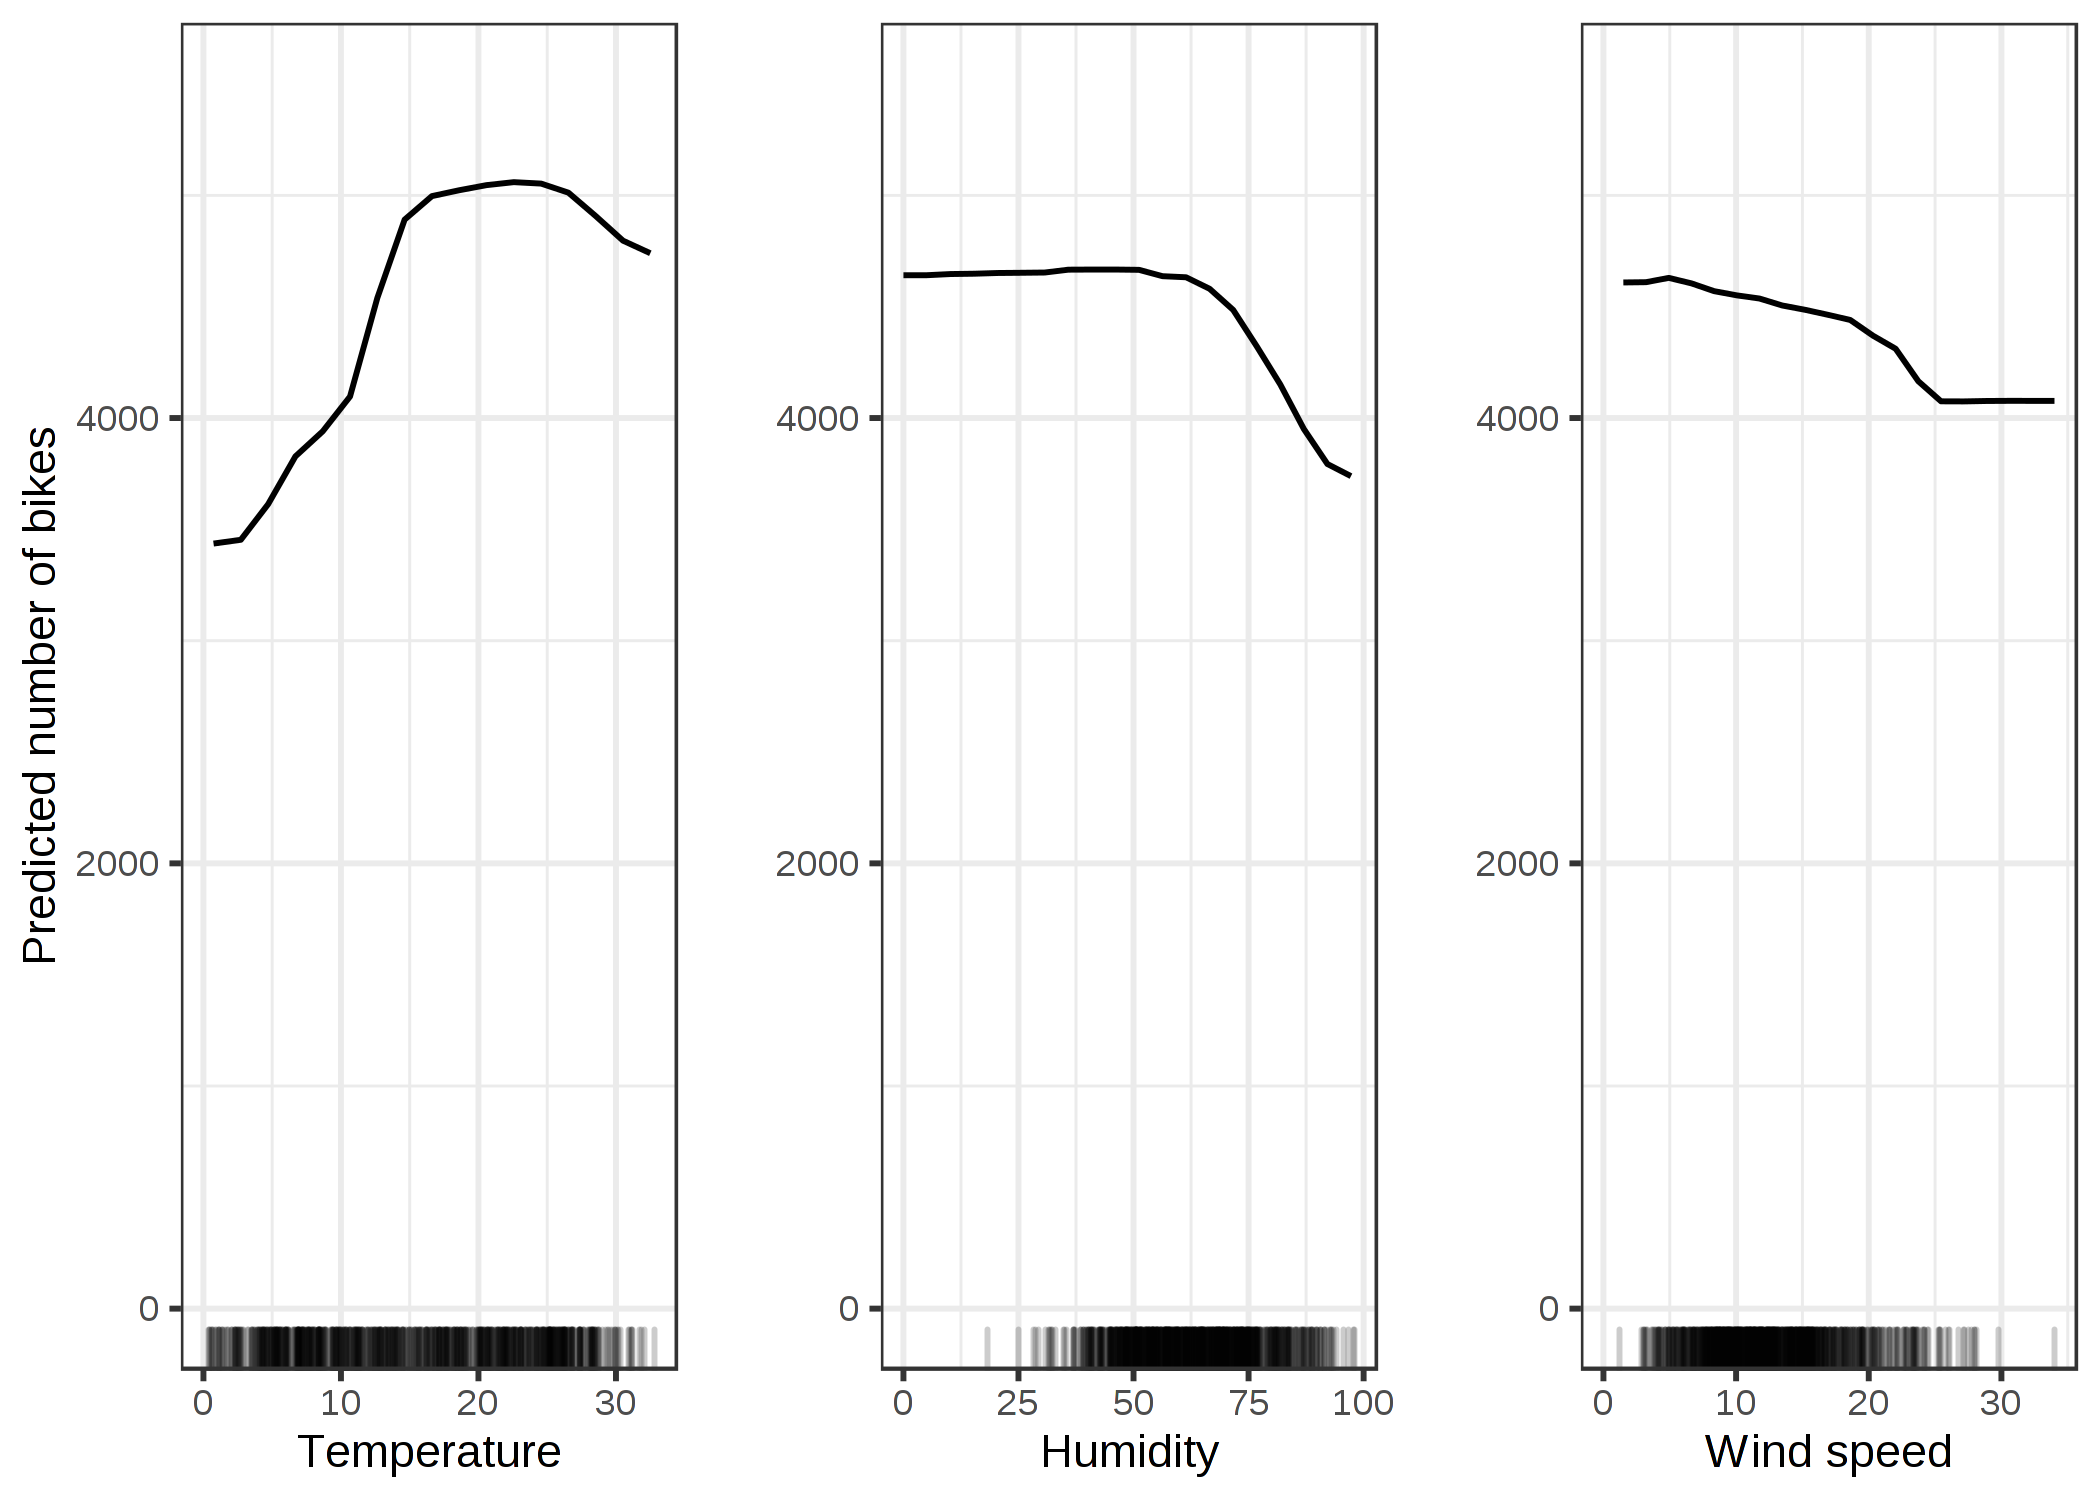
\includegraphics[scale=0.17]{src_img/partialDependencePlot.png}
        \caption{Exemple de diagramme de dépendance partielle.}
        \label{partialDependencePlot}
    \end{figure}
    
    \item \textbf{Sélection de prototype (Prototype Selection)} : Cet explicateur consiste à retourner, avec le résultat, un exemple très similaire à l'enregistrement classifié, afin de préciser avec quel critère la prédiction a été renvoyée.
    
    \item \textbf{Activation des neurones (Neurons Activation)} : L'analyse des réseaux de neurones permet aussi de comprendre son comportement. Cela consiste à analyser les neurones activés pour chaque entrés passées en argument à notre modèle.
\end{itemize}

L'explicateur varies en fonction de notre type de problème, de notre type de boite noire, de notre type de données d'entrée (images, texte...) et de nos différentes restrictions sur le modèle (accès au code, aux données...).

\section{Approches utilisées}
Face à ce besoin d'explicabilité grandissant, les entreprises peuvent préférer se tourner vers des modèles moins performant mais plus explicable afin de contourner la problématique de boite noire. Ainsi, nombreuse sont les entreprises qui se détournent de l'apprentissage profond au profil de l'apprentissage par arbre de décision ou les modèles linéaires par exemple qui fournissent un résultat plus compréhensibles et interprétable. Mais, la recherche dans ces domaines n'a pas évoluée depuis un certain temps et l'éventail des algorithmes disponibles est assez limité.

\subsubsection{Sur-couche explicative}
Le but étant d'essayer de fournir à l'utilisateur des éléments approximatifs permettant de comprendre son modèle boite noire, comme par exemple identifier les variables d'entrée les plus importantes dans la prise de décision du modèle. Comme le montre la figure 1.7, la sur-couche explicative vient se greffer après la prédiction du modèle.
\begin{figure}[h]
\centering
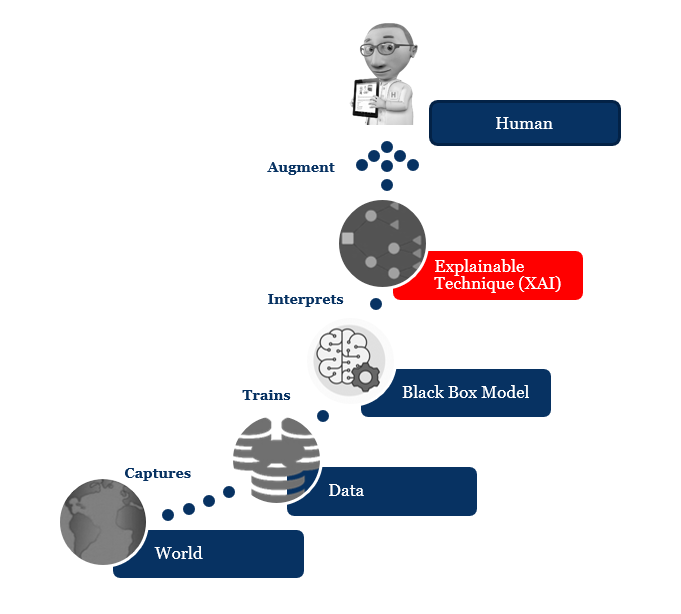
\includegraphics[scale=0.35]{src_img/explainCouche.png}
\caption{Position de la sur-couche explicative dans le processus de prédiction. \textit{Source : www.kdnuggets.com}}
\label{explainCouche}
\end{figure}
Différents outils proposent une approche permettant de livrer des éléments de compréhension approximatif pour un modèle boite noire simple. Nous allons présenter les deux outils les plus populaires, LIME et SHAP.
\subsection{LIME}
LIME signifie Local Interpretable Model-Agnostic Explanations (explications locales interprétables par modèle-agnostique). L'objectif est donc de fournir une interprétation local à un modèle de classification ou de régression (model agnostic) en se basant sur l’importance des variables comme vu précédemment. L'idée est de sonder la boite noire autant de fois que nécessaire en faisant varier les données d'entrées ce qui aura pour effet de produire une nouvelle sortie à chaque fois. Une fois toutes les perturbations sont effectuées il est alors possible de récupérer les coefficients qui composent la droite de la régression linéaire et ainsi de déduire l'importance des variables d'entrées. Par exemple dans la figure 1.8 tirée de l'article original de la présentation de LIME\cite{limePaper} : L'image originelle (a) est donnée à notre boite noire qui prédit "Guitare électrique", "Guitare acoustique" et "Labrador". Nous constatons que le modèle s'est trompé sur la reconnaissance de la guitare électrique et nous utilisons LIME afin de comprendre ce qu'il s'est passé. LIME va prendre notre image (a) et la dériver de plusieurs façons en cachant certaines parties et envoyer ces nouvelles images à notre modèle. Le but étant de trouver les parties qui une fois cachées font que le modèle ne prédit plus la même chose. Puis une fois les trois classes trouvées, LIME nous envoie une explication où l'on voit les parties de l'image aillant joué un rôle dans la prédiction de chaque labels de notre modèle.
\begin{figure}[h]
\centering
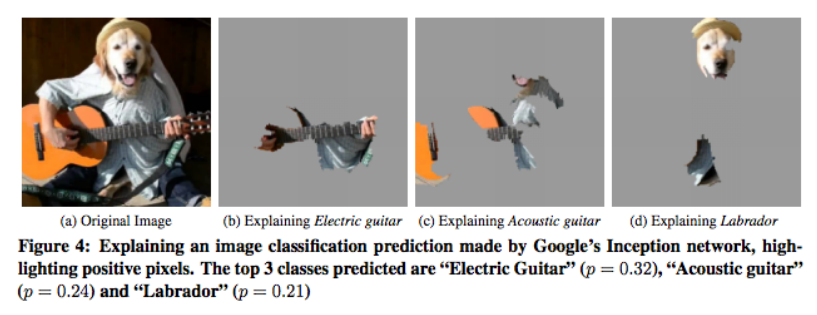
\includegraphics[scale=0.35]{src_img/limeExemple.png}
\caption{Source : LIME Paper}
\label{limeExemple}
\end{figure}

\subsection{SHAP}
Un an après la sortie de LIME, un nouvel outil fait son apparition afin de compenser ses quelques défauts, cet outil s'appelle SHAP. SHAP signifie SHapley Additive exPlanations, c'est une méthode permettant de fournir une interprétation local à une prédiction. Cette méthode est basée sur la valeur de Shapley issus de la théorie des jeux, il est donc nécessaire dans un premier temps d'expliquer brièvement cette valeur de Shapley.\par
La valeur de Shapley introduit par Shapley en 1953, permet de repartir les gains équitablement dans un jeu coopératif. Le but étant que tous les joueurs coopérant ensemble reçoivent un certain gain en fonction de leur contribution.\par
SHAP reprends cette idée afin d'expliquer toutes sortes de modèle de machine learning, le but étant d'associer une valeur égale à sa contribution dans la prédiction pour chaque caractéristique d'entrée. Prenons par exemple un modèle permettant de prédire le prix d'un logement. Une multitude de caractéristiques sont données en entrés à notre modèle afin d'estimer le prix du logement, le but de SHAP est donc de définir pour chacune de ces caractéristiques leur impact monétaire sur le prix final du logement. Il interrogera donc la boite noire avec une multitude de cas différents afin d'isoler le prix de chaque caractéristique. Prenons le cas de la figure 1.9 où l'on veut expliquer la prévision de 310 000 euros pour un logement de 50m2, au premier étage, près d'un parc et où les animaux sont interdits. SHAP va donc recréer la même l'instance et la donner en entrée à la boite noire en autorisant les animaux afin d'en déduire le coût (dans notre exemple 10 000 euros). Cette opération sera effectuée sur toutes les caractéristiques du problème afin de trouver la contribution de chacune. Cela peut sembler trivial dans cet exemple mais il peut exister des dépendances entre les caractéristiques qui modifient leurs coût en fonction de la présence ou non d'une ou plusieurs autre(s) caractéristique(s).
\begin{figure}[h]
\centering
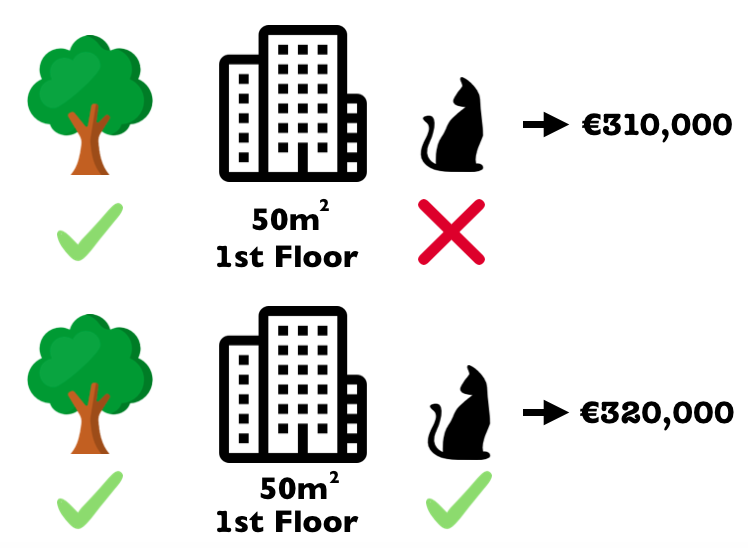
\includegraphics[scale=0.3]{src_img/shapleyExemple.png}
\caption{Exemple de l'explication du coût d'un logement avec SHAP. \textit{Source : Christoph Molnar, Interpretable Machine Learning}}
\label{shapleyExemple}
\end{figure}

\subsection{Limites de ces implémentations}
Aujourd'hui, de nombreuses implémentations de ces méthodes sont utilisées, mais elles essuient aussi quelques critiques et ne conviennent pas dans tous les cas de figures. Premièrement, ces algorithmes représentent un coût non négligeable. Ces méthodes basées sur des simulations et interrogeant notre modèle plusieurs fois pour une seule prédiction, peuvent poser des problèmes de performances lorsque l'on manipule un très grand nombre de données. Aussi la pertinence des explications fournies sont sujettes à débat, en effet ce sont des approximations et rien ne nous garantis que ces explications correspondent réellement au fonctionnement de notre modèle. Ces explications pourraient même donner l'effet inverse à celui escompté, en effet on peut arriver dans des cas où l'on fait confiance à notre modèle grâce à ces explications alors qu'elles ne sont pas fondées et ainsi prendre une décision critique appuyée sur une explication erroné.\par

Il est donc nécessaire d'utiliser ces algorithmes avec parcimonie et en aillant bien conscience qu'ils ne fournissent que des approximations de notre problème. Mais ce genre d'approches sont très bénéfiques pour la recherche, elles nous permettent d'apporter de nouvelles solutions ainsi que de mettre en lumière de nouvelles problématiques.
